


\section{Methodology}
\label{cp6:method}


To design an experiment
that examines how a tool that embeds a semantic-based technique might impact a developer's work,
we consider three main factors that might impact experimental design.




\paragraph{\textbf{Factors}}



To be helpful, a tool must direct a developer's attention to text that assist them complete a task~\cite{Robillard2015}. If we can gather data about the text in an artifact considered by humans as relevant to the task at hand, we should be able to assess whether the text automatically identified by the tool is \textit{similar} to the text manually identified. 


In case the text is not similar,
there is a chance that the tool directed a developer to the wrong information, or that 
the tool actually found complementary information that humans missed, which might impact the \textit{correctness} of a task. Therefore, our design must be able to compare the correctness of solutions submitted by participants who perform a task using our envisioned tool against that of developers who attempted the same tasks without tool support, i.e., a control group.


Regardless of how correct participants' solutions are, there is a chance that the text shown by the tool is not \textit{useful}---either because it is not relevant for the task at hand or because it is unsurprising, i.e., the information is ``common-knowledge'' to most developers~\cite{cwalina2008, Robillard2015}. Hence, a successful evaluation would 
also gather data that would allow us to discuss the usefulness of the text identified by the tool. 




\paragraph{\textbf{Design}}




Figure~\ref{fig:tool-experiment-procedures} presents an experiment that allows us to address the aforementioned factors. In this experiment, 24 participants with software development background each attempted a
\textit{manual task} and \textit{tool-assisted task} randomly drawn from a list of well-known Python programming tasks.
Alongside the solution submitted for each task, we use the manual task to collect what text participants deemed relevant to the task performed.
In turn, in the tool-assisted task, we also gathered input on the usefulness of the text automatically identified and shown by our tool. 
This design allow us to:




\begin{itemize}
    \item assess the correctness of the tasks performed \textit{with} or \textit{without} tool support;
    \item compare  the text that participants deemed relevant to the text automatically identified
    and shown in the tool-assisted task, and;
    \item discuss the usefulness of the automatically identified text according to the feedback provided by the participants.
\end{itemize}
 





\begin{figure}
\centering
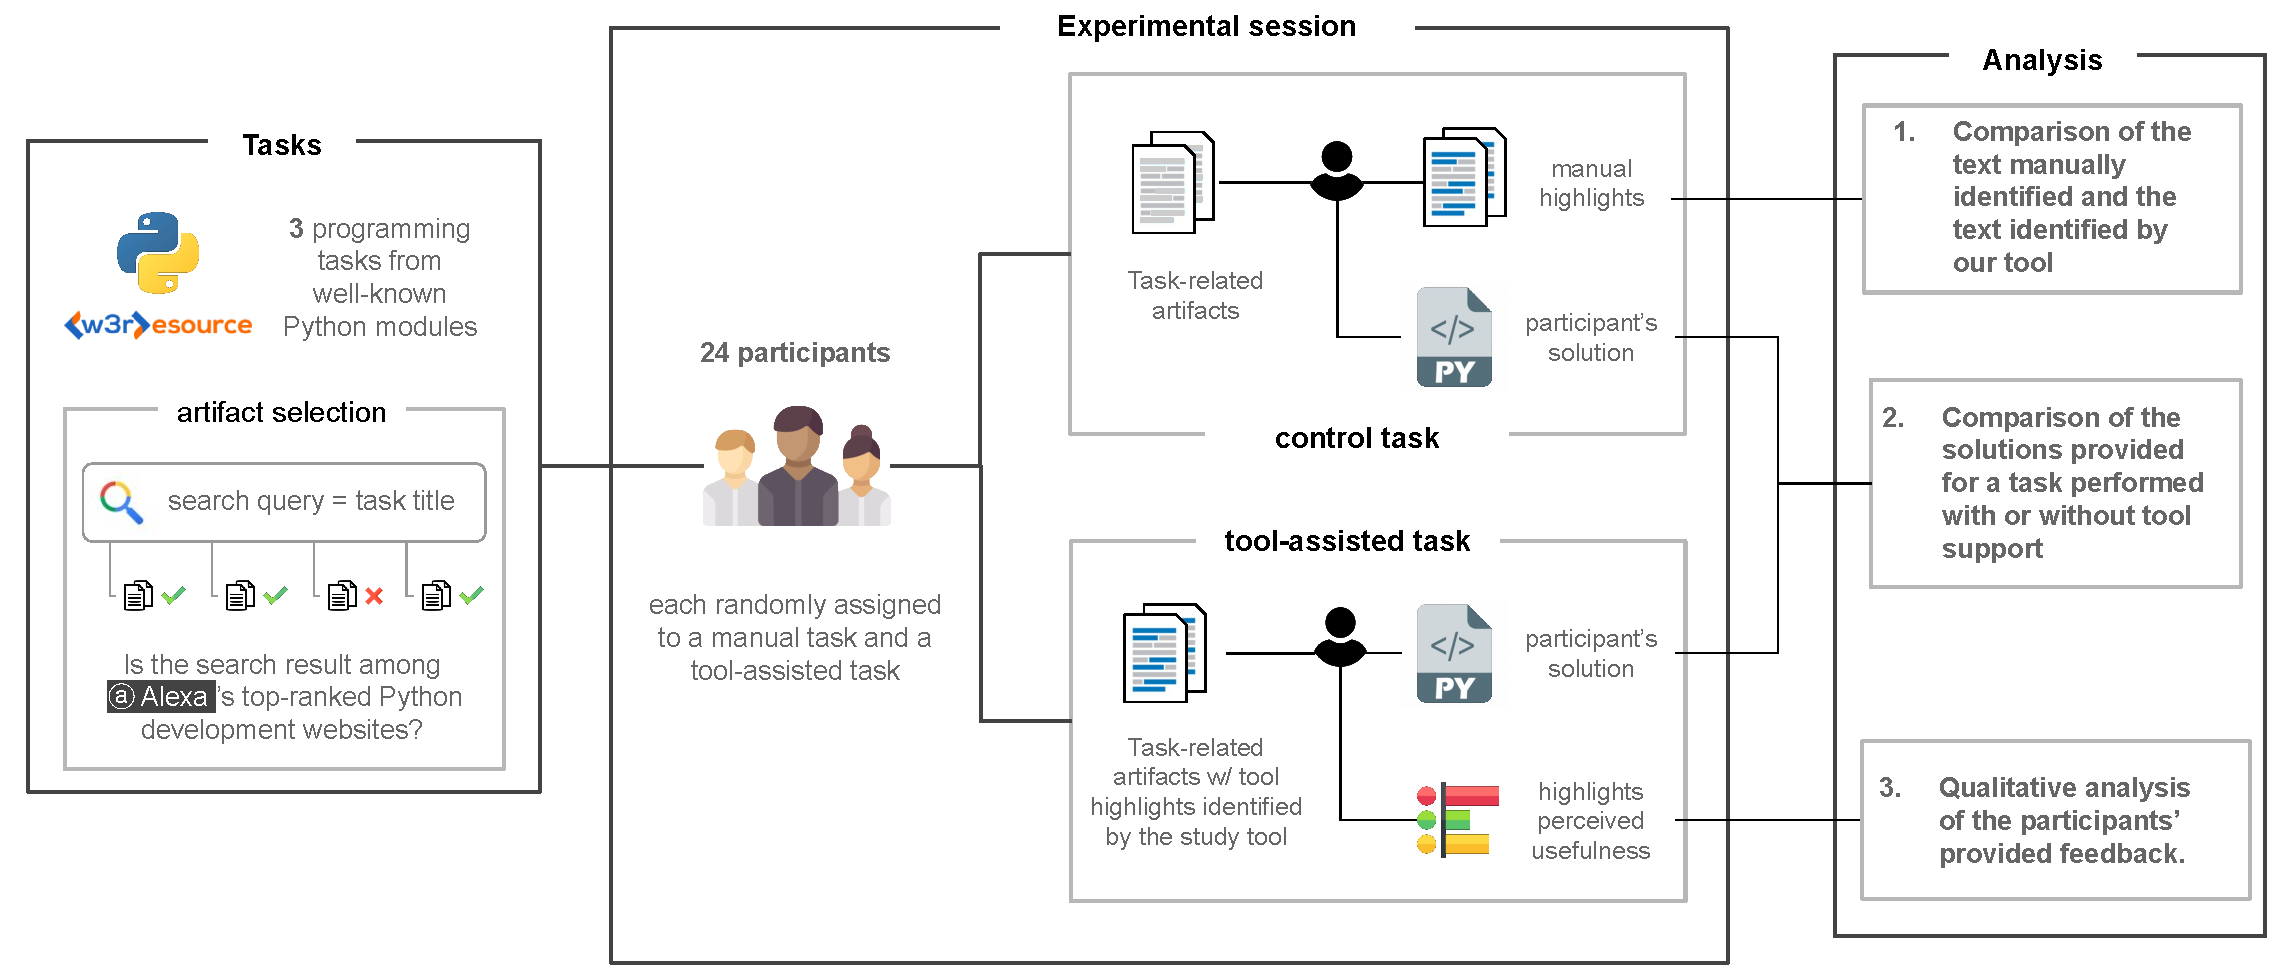
\includegraphics[width=1.05\textwidth]{cp6/tool-experiment-pipeline.pdf}
\caption{Summary of experimental procedures}
\label{fig:tool-experiment-procedures}
\end{figure}





\subsection{Tasks}
\label{cp6:tasks}


We opted for an experiment with tasks that could be completed by participants on their own time and computer.
This decision was motived by the COVID-19 pandemic and challenges related to recruiting participants and conducting an in-person experiment safely\red{~\cite{}}. 
Since participants would follow instructions on their own, we decided to use tasks that are easy to understand and perform in a single experimental session, but that still required a participant  
to seek information in artifacts associated with that task.



Based on these criteria and guided by~\cite{thiselton2019},
Table~\ref{tbl:python-tasks-modules} details the tasks that we have selected. 
These tasks are based on 
Python w3resource\footnote{\url{https://www.w3resource.com/python-exercises/}} tasks
that require usage of at least one module external to the Python core library.
By using external modules, we aim to reduce the likelihood that a participant 
can provide a solution for a task without consulting any of the artifacts (Section~\ref{cp6:coding-environment})
that detail how to use the modules associated with each task. 



While we leave details about the procedures associated with manual and tool-assisted tasks to another section, Figure~\ref{fig:nytimes-task-github} provides an excerpt of the information shown in a task\footnote{Full descriptions are available in the experiment's supplementary material~\red{\cite{}}.}.
For each task, participants had the task description and examples of input and output scenarios at their disposal. A task contained a list of resources that participants could consult 
so that they could write their solution.
Each task also contained a link to an online coding environment (Section~\ref{cp6:coding-environment})
where they could write and test their solution. 


\begin{table}
\centering
\caption{Python tasks}
\begin{footnotesize}
\rowcolors{2}{}{lightgray}
\begin{tabular}{ll}
\hline
\textbf{Task} & \textbf{Description}                                                                                         \\
\hline
\hline
%
\parbox[l][1cm][c]{1cm}{Practice task}       &
\parbox[l][1cm][c]{11cm}{Given three dictionaries representing address books,
you must write an algorithm using the Python core \texttt{dict} module to merge them.}    \\
\hline
%
Distances     &
\parbox[l][1.3cm][c]{11cm}{Given a string representing a rendezvou point and a list of suggested picnic addresses
    you must write an algorithm using the \texttt{geopy} module to find the  picnic address closest to the rendezvou point.} \\
%
NYTimes       &
\parbox[l][1cm][c]{11cm}{Given a string representing the url for NY Times Today's,
    write an algorithm using the \texttt{BeautifulSoup} and \texttt{requests} modules to scrape all the headlines of that page.}
\\
%
Titanic       &
\parbox[l][1cm][c]{11cm}{Given a string representing a url for the titanic dataset,
    you must write an algorithm using the \texttt{pandas} and \texttt{seaborn} modules to create a barchart of the data.}    \\
    
\hline
\end{tabular}
\end{footnotesize}
% \smallskip
\label{tbl:python-tasks-modules}
\end{table}




\subsection{Artifacts}
\label{cp6:experiment-artifacts}


Each task requires a set of artifacts that a participant could peruse for information that could assist them in writing their solution.
We select artifacts for a task following procedures similar to the ones we used to create the \acs{DS-android} dataset (Chapter~\ref{ch:android-corpus}). 
That is, for each of the tasks in Table~\ref{tbl:python-tasks-modules}, we use the Google search engine to obtain up to ten artifacts that likely contain 
information that could help a participant correctly complete that task. 


Note that our decision to control the artifacts shown per task relates to our need to study if there is overlap between the text that participants manually identify as relevant and the text that our semantic-based tool identifies for these same artifacts. 
Three pilot runs ensured that the artifacts available in each task had sufficient information to complete a task without 
the need of additional resources. 


\subsection{Coding environment}
\label{cp6:coding-environment}



To ensure that participants had the same conditions to perform each task
and also to minimize setup instructions, we used Google Colab\footnote{\url{https://colab.research.google.com/}} as our coding environment. 


Colab provided participants with a code editor with amenities commonly found in modern IDEs, e.g., code completion and syntax highlighting. It also ensured that all the participants 
performed the tasks in the same Python version and it lifted 
burdens that could arise from installing dependencies associated with the external modules used in each of our tasks. 


Figure~\ref{fig:nytimes-task-colab} shows an example of the Colab coding environment. 
First it handled dependencies management and then, 
it presented a class containing a single method with a \texttt{TODO} block where 
participants should write their solution. 
The environment also provided a main function where participants could see the output
of their code. Alternatively, a participant could use test cases to test their solution
against the examples shown in each task description.



\clearpage

\begin{figure}
    \centering
    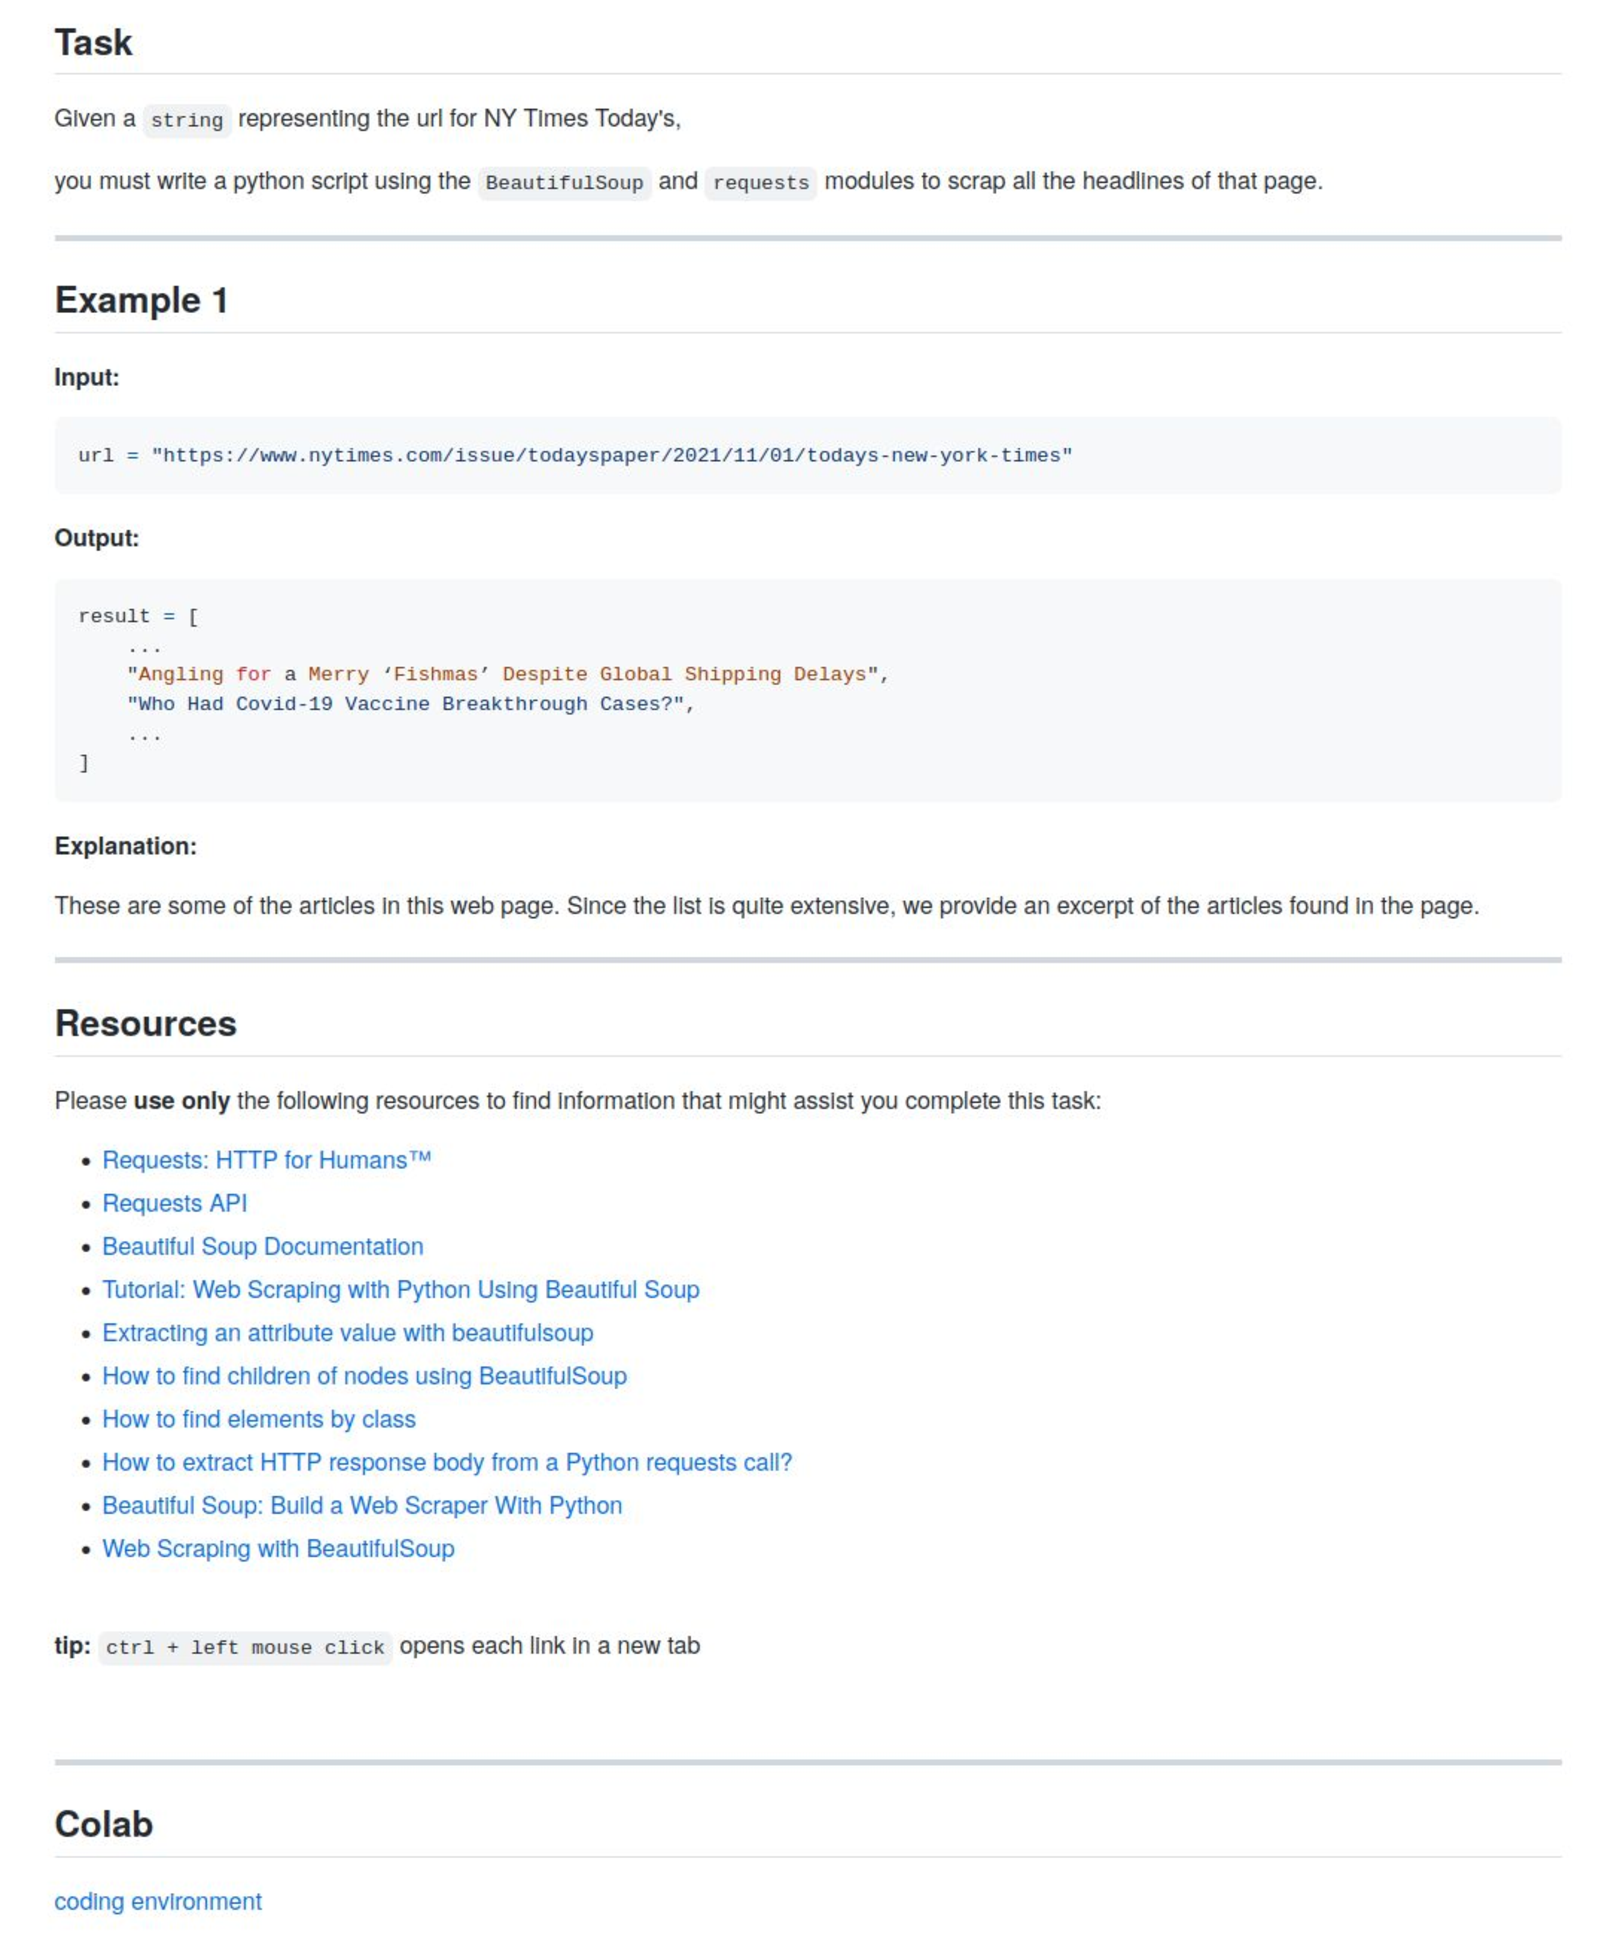
\includegraphics[width=1\textwidth]{cp6/task-github.pdf}
    \caption{Information shown in a task}
    \label{fig:nytimes-task-github}
\end{figure}



\clearpage

\begin{figure}
    \centering
    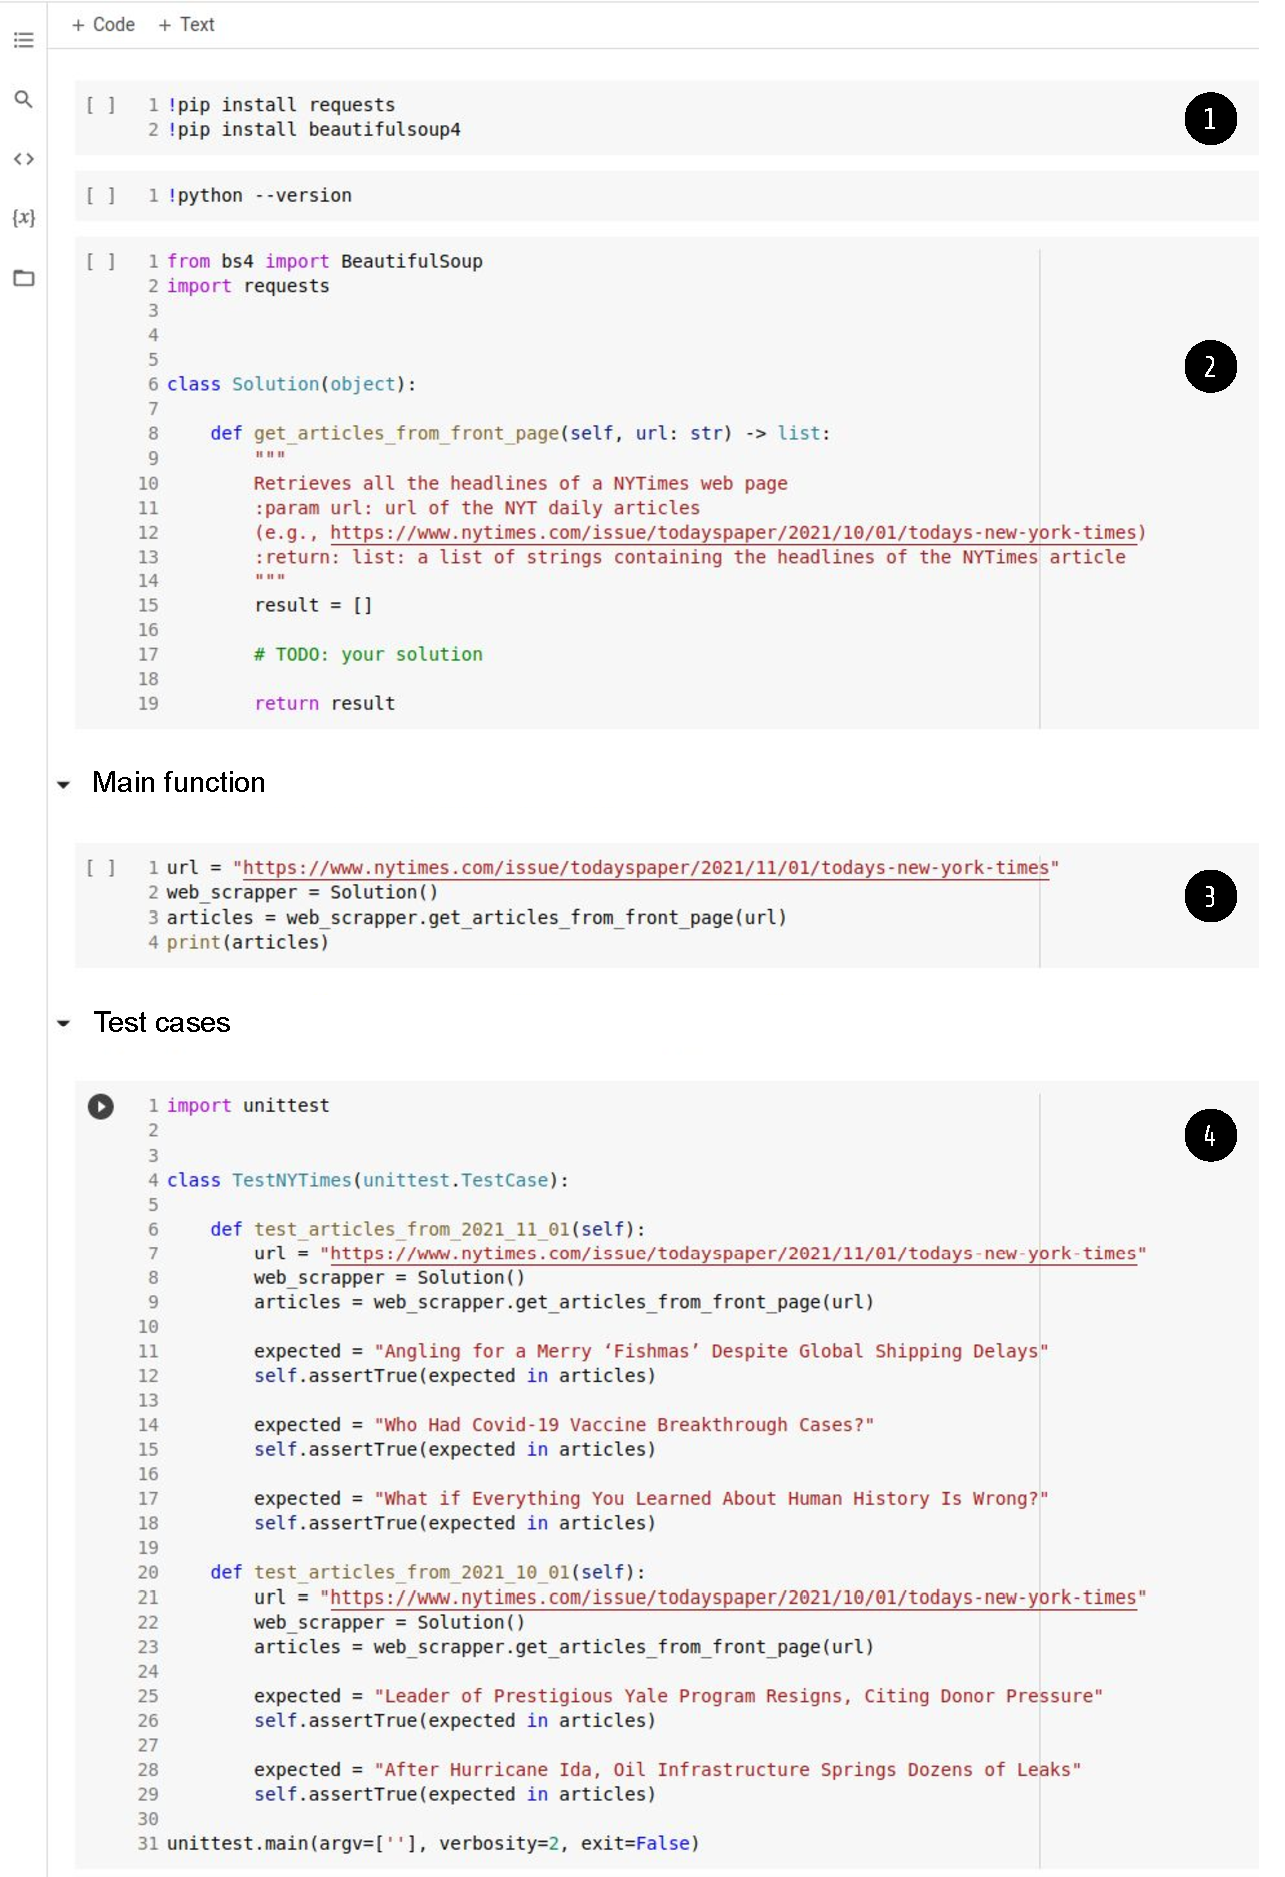
\includegraphics[width=\textwidth]{cp6/task-colab.pdf}
    \caption{Colab environment}
    \label{fig:nytimes-task-colab}
\end{figure}



\clearpage



\subsection{Participants}
\label{cp6:participants}


We advertised our study to professionals in our network and to computer science students at the several universities. 
Our target population comprised professionals and third, fourth-year or graduate students.
We expected participants to have experience in Object-Oriented programming languages, and to consult API documentation when performing a programming task. These questions were part of our demographics and we planned to exclude any participant
who did not meet these requirements. No participants were excluded
based on answers to these questions.




We obtained twenty four responses (3 identified female and 21 male) to our study advertisement. 
At the time of the experiment, 10 participants were working as software
developers and 14 were students (11 graduate and 3 undergrad).
We note that the majority of the students (71\%) also have previous professional experience.


On average, participants self-reported 8 years of programming experience ({\small $\pm$} 3.8, ranging from 3 to 17 years).
The majority of the participants (54\%) had between 5 to 10 years of experience in Object-Oriented programming languages,
closely followed by participants (29\%) with  3 to 4 years of experience.

